\documentclass{article}
% ============= Page size margins etc.
% ============= This offers great flexibility in terms of document size
\usepackage{geometry}
\geometry{twoside,
          letterpaper, % i.e, paperwidth=210mm and paperheight=297mm,
          top=35mm,
          bottom=40mm,
          left=25mm,
          right=25mm,
}
% =========== Math related stuff
% There are more tools for handling fractions etc.
% but can be left out until the need is obvious
\usepackage{mathtools} %<- Fixes, enhances amsmath package (loads amsmath too so no need to load it)
\usepackage{amssymb,amsthm}% Standard AMS tools

% =========== Graphics-related stuff
\usepackage{graphicx} % don't load epsfig or psfig
\usepackage[colorlinks = true,
            linkcolor = blue,
            urlcolor  = blue,
            citecolor = blue,
            anchorcolor = blue]{hyperref}

\usepackage{xcolor}


%Let's replicate the handout for demo, I'll call mytitle
\newcommand{\myTitleBox}{
\noindent\makebox[\linewidth][c]{%
  \colorbox{gray!30}{%
    \parbox{\paperwidth}{%
      \hspace*{\dimexpr\hoffset+\oddsidemargin+1in\relax}%
      \begin{minipage}{\dimexpr\textwidth-2\fboxsep-2\fboxrule\relax}
      {\centering\Large\topicsCovered\par}\vspace{2mm}
      \courseTitle\hfill\sectionTime\\
      \csname @author\endcsname\hfill\authorContact
      \end{minipage}
    }%
  }%
}
}

\setlength{\parskip}{1em}
\setlength{\parindent}{0pt}
% Now let's fill it up

\newcommand{\courseTitle}{APCOMP209a: Introduction to Data Science}
\newcommand{\sectionTime}{Wed 3-4pm \& Wed 5:30-6:30 \& Thurs 2:30-3:30}
\newcommand{\topicsCovered}{Bayesian Thinking and Linear Classification}
\newcommand{\authorContact}{nhoernle@g.harvard.edu}

\author{Nick Hoernle}


\begin{document}
\myTitleBox

\section{Bayesian Thinking}
%During the `hypothesis testing' section of Linear Regression, we saw a philosophy of reasoning where scientists present hypotheses, detail the assumptions that were made in presenting the hypotheses, and then evaluate the probability of observing the sampled data under those hypotheses. We have further seen that while certain  hypotheses can be rejected (as highly improbable), it is difficult to simply `accept' the alternative upon `rejecting' the null. In contrast to this approach, Bayesian statistics is concerned with evaluating the plausibility of an event given incomplete knowledge. In other words, instead of falsifying hypotheses using statistical tests, we rather employ an inductive approach of learning about general systems via the specific observations at hand and the beliefs of the scientist before obtaining the observed data \cite{gelman2013philosophy}.
During the `hypothesis testing' section of Linear Regression, we saw a philosophy of reasoning where we were presented with a sample from a `true' underlying statistical process. This sample of data represented a subset of data from the truth and we used hypothesis testing to evaluate the probability of the true parameters being different from a specific null hypothesis given the noisy and incomplete data. The specific observed data was the result of a random sampling procedure from a set of complete data (that would describe the model in its entirety). Bayesian Statistics takes a contrasting approach that dictates there is a distribution over the values that the parameters can hold given the fixed sample of data that we have observed. In this case, we consider the sample of data as fixed and rather try to understand what the specific sample implies for the probability of having a certain model.

% the sampling is no longer the random process but the actual system itself is a stochastic model. Considering the problem this way allows Bayesian data scientists to concern themselves with evaluating the plausibility of an event given incomplete knowledge.

% In other words they employ an inductive approach of learning about general systems via the specific observations at hand and the beliefs of the scientist before obtaining the observed data \cite{gelman2013philosophy}.

 % scientists present hypotheses, detail the assumptions that were made in presenting the hypotheses, and then evaluate the probability of observing the sampled data under those hypotheses. We have further seen that while certain  hypotheses can be rejected (as highly improbable), it is difficult to simply `accept' the alternative upon `rejecting' the null. In contrast to this approach, Bayesian statistics is concerned with evaluating the plausibility of an event given incomplete knowledge. In other words, instead of falsifying hypotheses using statistical tests, we rather employ an inductive approach of learning about general systems via the specific observations at hand and the beliefs of the scientist before obtaining the observed data \cite{gelman2013philosophy}.

We are interested in making conclusions about a model and its associated parameters ($\theta$) given some sample of data ($y$). Under a Bayesian framework, we consider the problem of understanding the probability distribution of the model parameters given the observed data, i.e. $p(\theta \vert y)$, and to do this, we must first consider the joint probability distribution for $\theta$ and $y$. The joint probability mass or density function can be factored into a multiplication of the \textit{prior distribution} $p(\theta)$ and the \textit{sampling distribution} $p(y \vert \theta)$. Using Bayes' rule, we can express the \textit{posterior} density in terms of the \textit{prior}, the \textit{sampling distribution} and the \textit{evidence or marginal likelihood} \cite{gelman2013philosophy} \cite{gelman2014bayesian}:
$$
p(\theta \vert y) = \frac{p(y \vert \theta)p(\theta)}{p(y)} = \frac{p(y \vert \theta)p(\theta)}{\int_{\theta}p(y \vert \theta)p(\theta)d\theta}\hspace{10px}\footnote{here we assume $p(y)$ is continuous and you should use a sum for the discrete case.}
$$

When the sampling distribution is considered a function of $\theta$ for a fixed $y$ (which in the Bayesian framework is the case) it called the \textit{likelihood function}.
% When optimising $p(y \vert \theta)p(\theta)$ (a function of $\theta$), it is common to ignore an often intractable $p(y)$ (constant with respect to the optimisation over $\theta$) and thus the simpler $p(\theta \vert y) \propto p(y \vert \theta)p(\theta)$ is used. From this relationship, the data $y$ can be seen to affect the posterior density only through $p(y \vert \theta)$ \cite{gelman2014bayesian}. When this quantity is considered a function of $\theta$ for a fixed $y$ (which in the Bayesian framework is the case) we give a different name to the \textit{sampling distribution} and call it the \textit{likelihood function}.

You have seen that when making classification decisions, we can evaluate the \textit{posterior odds} for different parameters $\theta_1$ and $\theta_2$ under a given model as:
$$
\frac{p(\theta_1 \vert y)}{p(\theta_2 \vert y)} = \frac{p(y \vert \theta_1)p(\theta_1)}{p(y \vert \theta_2)p(\theta_2)} = \frac{p(y \vert \theta_1)}{p(y \vert \theta_2)} \times \frac{p(\theta_1)}{p(\theta_2)}
$$
which is the same as saying the \textit{posterior odds} are equal to the \textit{prior odds} multiplied by the \textit{likelihood ratio}. This may look familiar from the Bayes' classifier from Logistic regression and we will return to it below when dealing with the LDA and QDA classifiers.

\section{Bayesian Interpretation of Lasso and Ridge Regression}
Refer to \href{https://github.com/cs109/a-2017/blob/master/Sections/advanced/sec3.pdf}{Week 3 Advanced Section Notes} - Section 5 Bayesian Interpretation of Ridge and Lasso Regression.

\section{Fisher's Linear Discriminant}
In \href{https://github.com/cs109/a-2017/blob/master/Sections/advanced/sec4.pdf}{Section 4} we discussed the dimensionality reduction method of Principal Component Analysis (PCA). Similarly, Linear Discriminant Analysis (LDA) can be thought of as a dimensionality reduction technique where a linear discriminant is found that attempts to maximally separate two different classes. PCA, under its assumptions, attempts to find the Principal Components that account for most of the variance in the dataset. On the other hand, LDA attempts to model the difference between the classes of data.\footnote{It is worth noting LDA is a supervised technique whereas PCA is unsupervised even though, in this case, we are comparing them for the same function of dimensionality reduction.}

Let's imagine an example in two dimensions with data belonging to one of two classes, where the two classes have (Gaussian) marginal distributions that are highly elongated but aligned (see figure \ref{fig:lda_vs_pcs_ex} for an example).
\begin{figure}[h]
\center
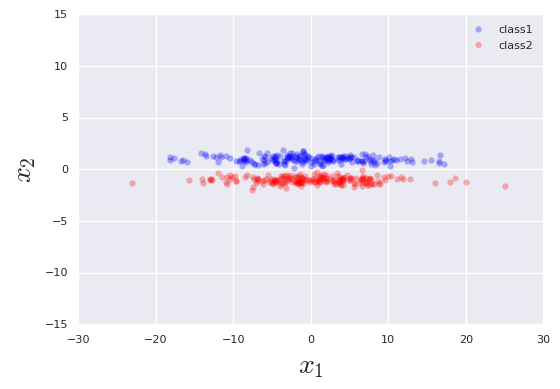
\includegraphics[width=8cm]{lda_vs_pcs_ex}
\caption{Example dataset where LDA will present a more useful dimensionality reduction than PCA}\label{fig:lda_vs_pcs_ex}
\end{figure}
As you learnt, the first principal component will extract the dimension that captures the highest variance in the data (in this case it will be exactly $x_1$). For the purposes of dimensionality reduction, projecting the data onto this component will actually result in a one dimensional representation where the data is entirely inseparable (see figure \ref{fig:pca_projection}).\footnote{For the purposes of visualising the data, I have added a small amount of vertical jitter for plotting the points.}

\begin{figure}[h]
\center
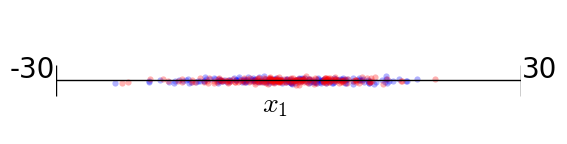
\includegraphics[width=8cm]{pca_projection}
\caption{Example of a projection that does not discriminate between the data classes}\label{fig:pca_projection}
\end{figure}

We can clearly see that for the task of classification, a much more useful projection would be one onto the $x_2$ component. Fisher Linear Discriminant Analysis (LDA) considers maximising an objective with the goal of finding a \textit{discriminating} hyperplane between these classes \cite{welling2005fisher} (and not the hyperplane that describes the variance of the dataset in its entirety). LDA uses the additional information of known class labels to find a more useful discriminator between the data classes. To achieve this, Fisher LDA attempts to project the class means onto some subspace $\mathbf{W}$ such that the distance between the means is maximised while the variance of the data within each of the classes is minimised. $\mathbf{W}$ can be thought of as consisting of column vectors $\mathbf{w}$ that each represent a hyperplane that discriminates between two classes. To do this, we need the \textit{between-class scatter} matrix \footnote{there are $k$ classes and $i \in k$ is the index of a datapoint belonging to the the $k^{th}$ class. Moreover, $\mu_k$ is the mean of class $k$, $x_i$ is a datapoint and $\bar{x}$ is the mean of the entire dataset.}$S_B = \sum_k(\mathbf{\mu_k - \mathbf{\bar{x}}})(\mathbf{\mu_k - \mathbf{\bar{x}}})^T$ (measuring the spread of the class means) and the \textit{total within-class scatter} matrix $S_W = \sum_k \sum_{i \in k}(\mathbf{x_i} - \mathbf{\mu_k})(\mathbf{x_i} - \mathbf{\mu_k})^T$. The optimisation task is then to find the vector $\mathbf{w}$ that maximises the following objective (also called the Rayleigh quotient):

$$
J(\mathbf{w}) = \frac{\mathbf{w}^TS_B\mathbf{w}}{\mathbf{w}^TS_W\mathbf{w}}
$$

Studying the two class case is helpful: let's assume we have data from two Gaussian distributions $(X|Y=1) \sim N(\mu_1, \Sigma_1$) and $(X|Y=2) \sim N(\mu_2, \Sigma_2$) for classes $1$ and $2$ respectively. We have $S_B = (\mu_1 - \mu_2)(\mu_1 - \mu_2)^T$ and $S_W = (\Sigma_1 + \Sigma_2)$.

Maximising the objective $J$ with respect to $\mathbf{w}$ is equivalent to maximising the numerator while holding the denominator constant (and as we are only interested in the direction of $\mathbf{w}$, we can hold the denominator constant to $1$). So we find $\mathbf{w}$ to $max (\mathbf{w}^TS_B\mathbf{w})$ such that $\mathbf{w}^TS_W\mathbf{w} = 1$ which results in the following Legrangian:

$$
L = \mathbf{w}^T S_B\mathbf{w} + \lambda(\mathbf{w}^T S_W\mathbf{w} - 1)
$$

Setting $\frac{\partial L}{\partial \mathbf{w}}$ to $0$ yields $2(S_B - \lambda S_W)\mathbf{w} = 0$ and so:

\begin{equation}
  S_W^{-1}S_B \mathbf{w} = \lambda \mathbf{w}
\end{equation}

In general the solution exists if $S_W^{-1}$ exists. Moreover, the solution is not unique and corresponds to the eigenvalue problem for the $S_W^{-1}S_B$ matrix.

Referring back to the two class case, and using the definition of $S_B$, we see that
$$
S_W^{-1}S_B \mathbf{w} = S_W^{-1}(\mu_1 - \mu_2)(\mu_1 - \mu_2)^T \mathbf{w} = \lambda \mathbf{w}
$$and finally noting that $(\mu_1 - \mu_2)^T \mathbf{w}$ is a scalar we get:
\begin{equation}
  S_W^{-1} (\mu_1 - \mu_2) = \frac{\lambda}{\alpha} \mathbf{w}
\end{equation}

Again, we are only interested in the direction of $\mathbf{w}$ (and can discard the scalar multiplier), so
$$
\mathbf{w^*} = S_W^{-1} (\mu_1 - \mu_2)
$$

In the more general case where we have $K$ classes (and $K$ associated means $\mu_k$), with $K \geq 2$, this space can only span $K-1$ dimensions. In otherwords, we can, in theory, project any datapoint $x$ onto the $K-1$ dimensional space spanned by the $K$ centroids (i.e. classify the data to one of the classes) and not lose any information. Moreover, studying $rank(S_W^{-1}S_B) \leq \min\{ rank(S_W^{-1}), rank(S_B) \}$, \cite{petersen2008matrix} and asserting that $rank(S_B) < K-1$, we have $rank(S_W^{-1}S_B) \leq K-1$. So LDA projects a p dimensional vector onto a $K-1$ dimensional subspace for which the data is maximally (linearly) separated.

% and we consider the space that is spanned by the mean vectors for each of the classes, these vectors only span a space of $K-1$ dimensions. it can be shown that $S_W^{-1}S_B$ is of rank $K-1$.

% Where $S_B = \sum_k(\mathbf{\mu_k - \mathbf{\bar{x}}})(\mathbf{\mu_k - \mathbf{\bar{x}}})^T$ and $S_W = \sum_k \sum_{i \in k}(\mathbf{x_i} - \mathbf{\mu_k})(\mathbf{x_i} - \mathbf{\mu_k})^T$. I.e. $S_B$ is the scatter matrix between the cluster means (\textit{between-class scatter} matrix) and $S_W$ is the \textit{total within-class scatter} matrix (with $\mathbf{\bar{x}}$ referring to the overall mean of the dataset). Minimising this objective is intuitively finding a vector $\mathbf{w}$ such that the class-means are well separated, measured relative to the (sum of the) variances of the data within each class.
% Note that finding $\mathbf{w}$ only depends on the direction of the vector and not the magnitude (i.e. the objective $J$ is invariant with respect to magnitude scalings of the vector $\mathbf{w}$). Setting the gradient to 0, $\frac{\partial J}{\partial \mathbf{w}} = 0$, yields $(\mathbf{w}S_B\mathbf{w})S_W\mathbf{w} = (\mathbf{w}S_W\mathbf{w})S_B\mathbf{w}$. Here, you should notice that $(\mathbf{w}S_B\mathbf{w})$ and $(\mathbf{w}S_W\mathbf{w})$ are constants \footnote{write out the matrix dimensions if you are not convinced of this.} so:
%
% $$
% \lambda S_W\mathbf{w} = S_B\mathbf{w}
% $$
%
% and $S_W^{-1}S_B\mathbf{w} = \lambda\mathbf{w}$. You should recognise this as an eigenvalue problem of $S_W^{-1}S_B$ with eigenvectors $\mathbf{w_i}$ and associated eigenvalues $\lambda_i$. A worthwhile exercise is to use the fact that $J$ is invariant with respect to magnitude scalings of the vector $\mathbf{w}$ to choose $\mathbf{w}$ such that the denominator of J is set to 1. This is then the constrained optimisation problem\cite{welling2005fisher}:
% $min_{\mathbf{w}} (-\frac{1}{2}\mathbf{w}^TS_B\mathbf{w})$ such that $\mathbf{w}^TS_W\mathbf{w} = 1$.\footnote{the $\frac{1}{2}$ in this equation is included for convenience in the optimisation task.}
%
% Fisher showed\cite{fisher1938statistical} that if $S_W$ is nonsingular, then you can construct a projection matrix $W$ which has the eigenvectors of $S_W^{-1}S_B$ as its columns.


\begin{figure}[h]
\center
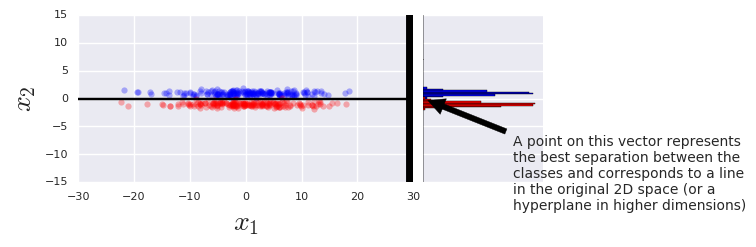
\includegraphics[width=15cm]{best_projection}
\caption{Example of a projection that does discriminate between the data classes}\label{fig:best_proj}
\end{figure}

%Asside: In this case, with $\mathbf{w}$ the optimal projection vector for maximally separating the class, we would project $\mathbf{x}$ onto $\mathbf{w}$ y = $\mathbf{w}^Tx$, and make a classification decision based on $y \geq w_o$. You would use Decision theory to decide on $w_o$ that minimises the misclassification rate.

\section{LDA and QDA Classifiers}
We can now tackle the same problem of discriminating among the data classes, but use properties of Gaussian distributions and the posterior odds of a datapoint originating from a certain class specific distribution. From classification Decision theory, we know that to minimise the misclassification rate, it is optimal to classify a datapoint to the most probable class using the posterior probability $P(Y|X)$, where $Y$ denotes the classification decision and $X$ denotes the predictors in the model (refer to the \textit{Bayes Classifier} discussed in class). If we let $f_k(x)$ denote the class-conditional density of X in the class Y=k, and we let $\pi_k$ be the prior probability that a datapoint chosen at random will be observed as class k (note that $\sum_{k=1}^K \pi_k = 1$) then we have:
$$
p(Y=k|X=x) = \frac{p(X=x|Y=k)p(Y=k)}{p(X=x)} = \frac{f_k(x) \pi_k}{\sum_{l=1}^K f_l(x) \pi_l}
$$
the denominator follows from the law of total probability. We make the explicit assumption that the densities $f_k(x)$ follow multivariate Gaussian distributions (i.e. $(X|Y=k) \sim N(\mu_k, \Sigma_k)$) which means that the densities follow:

$$
f_k(x) = \frac{1}{(2\pi)^{p/2} \vert \Sigma_k \vert ^{1/2} } \exp \big \{\frac{-1}{2}(x - \mu_k)^T \Sigma_k^{-1} (x - \mu_k) \big \}
$$

Classifying a new datapoint to the class with the highest posterior probability, $max(p(Y|X)) = max(\log [p(Y|X)])$, results in classifying the datapoint to the class that maximises:
$$
\delta_k(x) = log(\pi_k) - \frac{1}{2}log(\vert \Sigma_k \vert) - \frac{1}{2}(x - \mu_k)^T \Sigma_k^{-1} (x - \mu_k)
$$

Notice that $(x - \mu_k)^T \Sigma^{-1} (x - \mu_k)$ is the squared Mahalanobis distance metric. Further note that for the two class problem (with class 1 and class 2), $\delta_1(x) = \delta_2(x)$ represents the decision boundary between the two classes, and this decision boundary is quadratic in $x$ (\textit{refer to your lecture notes for more on this topic}).

Dealing with the case that the classes have the same (pooled) covariance matrices, we have the objective of classifying the datapoint to the class that maximises:
$$
\delta_k(x) = x^T \Sigma^{-1}\mu_k + log(\pi_k) -\frac{1}{2}\mu_k^T\Sigma^{-1}\mu_k
$$

Again, for the two class problem, we can look at the log posterior-odds:
$$
\frac{p(Y=k \vert X=x)}{p(Y=l \vert X=x)} = \frac{f_k(x)\pi_k}{f_l(x)\pi_l} = log\frac{\pi_k}{\pi_l} - \frac{1}{2}(\mu_k+\mu_l)^T\Sigma^{-1}(\mu_k-\mu_l) + x^T \Sigma^{-1}(\mu_k - \mu_l)
$$
Note now that the decision boundary would be linear in $x$. Further note that the $\Sigma^{-1}(\mu_k - \mu_l)$ direction term is the same as the $\mathbf{w}$ vector found above.


\section{Notes}
\begin{enumerate}
  \item LDA/QDA classifies a new datapoint to the class with the closest centroid. Here `closest' is measured in the Mahalanobis metric, using a pooled covariance estimate.
  \item Under the assumption that the data are multi-variate Gaussian within each class, LDA is a Bayes' classifier (i.e. it minimises the probability of making a mis-classification).
  \item LDA results in linear decision boundaries.
  \item In many cases, when linear decision boundaries are inadequate for separating the classes, QDA can be used, with the cost of needing to estimating more parameters.
  \item LDA needs to approximate the following ($K + K + P^2$) statistics from the data\footnote{Here I use $i \in k$ to denote the index of datapoint $i$ that belongs to class $k$.}:
  \begin{enumerate}
    \item K priors: $\hat\pi_k = \frac{N_k}{N}$
    \item K means: $\hat\mu_k = \sum_{i \in k} \frac{x_i}{N_k}$
    \item 1 covariance matrix: $\hat\Sigma = \sum_{k=1}^K\sum_{i \in k} \frac{(x_i - \hat\mu_k)(x_i - \hat\mu_k)^T}{N-K}$
  \end{enumerate}
  \item QDA needs to approximate the following ($K + K + K \times P^2$) statistics from the data (notice the possibility for overfitting your training data here):
  \begin{enumerate}
    \item K priors: $\hat\pi_k = \frac{N_k}{N}$
    \item K means: $\hat\mu_k = \sum_{i \in k} \frac{x_i}{N_k}$
    \item K covariance matrices: $\hat\Sigma_k = \sum_{i \in k} \frac{(x_i - \hat\mu_k)(x_i - \hat\mu_k)^T}{N_k}$
  \end{enumerate}
\end{enumerate}

Other interesting and worthwhile references are: \cite{turk1991face}, \cite{belhumeur1997eigenfaces}, \cite{martinez2001pca}.

\bibliography{section_6}
\bibliographystyle{ieeetr}

\end{document}
